\csname @openrightfalse\endcsname
\chapter{Surfaces}

We assume that the reader is familiar with smooth surfaces and the related definitions
including intrinsic metric, 
geodesics,
convex and saddle surfaces
as well as different types of curvature.
An introductory course in differential geometry should cover all necessary background material 
[see for example \S28--29 in \ncite{hilbert-cohn-vossen}
or  
\ncite{toponogov-curves-and-surfaces}].



%%%%%%%%%%%%%%%%%%%%%%%%%%%%%%%%%%%%%%%%%%%%%%
{

\begin{wrapfigure}{r}{27 mm}
\vskip4mm
\centering
\includegraphics{mppics/pic-202}
\end{wrapfigure}


\subsection*{Convex hat}
\label{Convex hat}

\begin{pr}
Suppose that a plane $\Pi$ cuts from a smooth closed convex surface $\Sigma$ a disk $\Delta$.
Assume that the reflection of $\Delta$ with respect to $\Pi$ lies inside of $\Sigma$.
Show that $\Delta$ is \index{convex set}\emph{convex} with respect to the intrinsic metric  of $\Sigma$;
that is, 
if both ends of a minimizing geodesic in $\Sigma$ 
lie in $\Delta$,
then the entire geodesic lies in $\Delta$.
\end{pr}

}


\parit{Semisolution.}
Assume the contrary,
then there is a minimizing geodesic $\gamma\not\subset\Delta$ with ends $p$ and $q$ in $\Delta$.

Without loss of generality, we may assume that only one arc of $\gamma$ lies outside of $\Delta$.
Reflection of this arc  with respect to $\Pi$ together with the remaining part of $\gamma$ forms another curve $\hat\gamma$ from $p$ to $q$;
it runs partly along $\Sigma$ 
and partly outside $\Sigma$,
but does not get inside $\Sigma$.
Note that
\[\length\hat\gamma=\length\gamma.\]


Denote by $\bar\gamma$ the closest point projection of $\hat\gamma$ on $\Sigma$.
Since $\Sigma$ is convex, the closest point projection decreases the length.
Therefore 
the curve $\bar\gamma$ lies in $\Sigma$, 
it has the same ends as $\gamma$,
and
\[\length\bar\gamma<\length\gamma.\]
This means that $\gamma$ is not length minimizing, 
a contradiction.\qeds

%%%%%%%%%%%%%%%%%%%%%%%%%%%%%%%%%%%%%%%%%%%%%%

{


\begin{wrapfigure}{r}{39 mm}
\vskip0mm
\centering
\includegraphics{mppics/pic-204}
\end{wrapfigure}

\subsection*{Involute of geodesic}
\label{Involute of  geodesic}

\begin{pr}
Let $\Sigma$ be a smooth closed strictly convex surface 
in $\RR^3$ 
and $\gamma\:[0,\ell]\z\to \Sigma$ a unit-speed minimizing geodesic.
Set $p\z=\gamma(0)$, $q=\gamma(\ell)$ and 
$$p_t=\gamma(t)-t\cdot\gamma'(t),$$ 
where $\gamma'(t)$ denotes the velocity vector of $\gamma$ at $t$.
\end{pr}

}
\vskip-\medskipamount
\textit{Show that for any $t\in (0,\ell)$,
one {}\emph{cannot see}  $q$ from $p_t$;
that is, the line segment $[p_tq]$ intersects $\Sigma$ at a point distinct from $q$.}

%%%%%%%%%%%%%%%%%%%%%%%%%%%%%%%%%%%%%%%%%%%%%%
\subsection*{Simple geodesic}
\label{Simple geodesic}

\begin{pr}
Let $\Sigma$ be a complete unbounded convex surface in $\mathbb R^3$.
Show that there is a two-sided infinite geodesic in $\Sigma$ with no self-intersections.
\end{pr}

Let us review a couple of statements 
about Gauss curvature which might help to solve the problem \cite[see \S28 in][for more details]{hilbert-cohn-vossen}.

If $\Sigma$ is a convex surface in $\RR^3$ then its Gauss curvature is nonnegative.

Assume that a simply connected region $\Omega$ in the surface $\Sigma$ is bounded by a closed broken geodesic $\gamma$.
Denote by $\kappa(\Omega)$ the integral of the Gauss curvature over $\Omega$.

For any point $p\in\Sigma$ consider the outer unit normal vector $n(p)\z\in\mathbb{S}^2$.
Then 
\begin{align*}
\kappa(\Omega)&=\area[n(\Omega)]
\intertext{and by the Gauss--Bonnet formula}
\kappa(\Omega)&=2\cdot\pi-\sigma(\gamma),
\end{align*}
where $\sigma(\gamma)$ denotes the sum of the signed exterior angles of $\gamma$.
In particular,  $|\sigma(\gamma)|\le2\cdot\pi$.





%%%%%%%%%%%%%%%%%%%%%%%%%%%%%%%%%%%%%%%%%%%%%%
\subsection*{Geodesics for birds}
\label{liberman}

The \index{total curvature}\emph{total curvature} of a space curve $\gamma$ is defined as the integral of its curvature.
That is, if a curve $\gamma\:[a,b]\to\RR^3$ has unit speed parametrization, 
then its total curvature equals 
\[\int\limits_a^b|\gamma''(t)|\cdot dt,\]
the vector $\gamma''(t)$ is called \index{curvature vector}\emph{curvature vector} and its length $|\gamma''(t)|$ is the \index{curvature}\emph{curvature} of $\gamma$ at time $t$.
The above definition makes sense for $C^{1,1}$ smooth curves,
that is, in the case when $\gamma'(t)$ is locally Lipschitz;
in this case the curvature $|\gamma''(t)|$ is defined almost everywhere.

The \index{geodesic}\emph{geodesics} in the following problem are defined as the curves locally minimizing the length;
that is, any sufficiently short arc of the curve containing a given value of the parameter is length minimizing.

\begin{pr}
Let $f\:\RR^2\to\RR$ be a smooth $\ell$-Lipschitz function.
Let $W\subset \RR^3$ be the epigraph of $f$;
that is,
$$W=\set{(x,y,z)\in\RR^3}{z\ge f(x,y)}.$$
Equip $W$ with the induced intrinsic metric.

Show that any geodesic in $W$ 
 has  total curvature at most $2\cdot\ell$. 
\end{pr}

Actually, geodesics in $W$ are $C^{1,1}$-smooth;
in particular, the formula for the total curvature mentioned above makes sense.
This is an easy exercise in real analysis which can be also taken for granted.


%%%%%%%%%%%%%%%%%%%%%%%%%%%%%%%%%%%%%%%%%%%%%%
\subsection*{Immersed surface}
\label{Immersed surface}

\begin{pr}
Let $\Sigma$ be a smooth connected immersed surface in $\RR^3$ with strictly positive Gauss curvature and nonempty boundary $\partial\Sigma$.
Assume that the boundary $\partial\Sigma$ lies in a plane $\Pi$
and $\Sigma$ lies entirely in one side of~$\Pi$.
Prove that $\Sigma$ is an embedded disk.
\end{pr}

%%%%%%%%%%%%%%%%%%%%%%%%%%%%%%%%%%%%%%%%%%%%%%
\subsection*{Periodic asymptote}
\label{Asymptotic geodesic}

\begin{pr}
Let $\Sigma$ be a closed smooth surface with non-positive curvature at every point
and $\gamma$ a geodesic in $\Sigma$.
Assume that $\gamma$ is not periodic
and the curvature of $\Sigma$ vanishes at every point of $\gamma$.
Show that $\gamma$ does not have a periodic asymptote;
that is, there is no periodic geodesic $\delta$ such that the distance from $\gamma(t)$ to $\delta$  converges to $0$ as $t\to\infty$. 
\end{pr}

%%%%%%%%%%%%%%%%%%%%%%%%%%%%%%%%%%%%%%%%%%%%%%
\subsection*{Saddle surface}
\label{Saddle surface}

Recall that a smooth surface $\Sigma$ in $\RR^3$
is \index{saddle surface}\emph{saddle} at a point $p$ if its principal curvatures at $p$ have opposite signs. 
We say that $\Sigma$ is {}\emph{saddle} if it is saddle at all points.

\begin{pr}
Let $\Sigma$ be a saddle surface in $\RR^3$
homeomorphic to a disk.
Assume that the orthogonal projection to the $(x,y)$-plane
maps the boundary of $\Sigma$
injectively to a convex closed curve.
Show that the orthogonal projection to $(x,y)$-plane is injective on $\Sigma$.

In particular, $\Sigma$ is the graph $z=f(x,y)$ of a function $f$ defined on a convex domain in the $(x,y)$-plane.
\end{pr}


%%%%%%%%%%%%%%%%%%%%%%%%%%%%%%%%%%%%%%%%%%%%%%
\subsection*{Asymptotic line}
\label{asymptotic-line}

The saddle surfaces are defined in the previous problem.

Recall that a smooth curve $\gamma$ on a smooth surface $\Sigma\subset \RR^3$ is called \index{asymptotic line}\emph{asymptotic line} if $\gamma''(t)$ is tangent to the surface at $\gamma(t)$ for any $t$.

\begin{pr}
Let $\Sigma\subset \RR^3$ be the graph $z\z=f(x,y)$
of a smooth function $f$ 
and $\gamma$ a closed smooth asymptotic line in $\Sigma$.
Assume that $\Sigma$ is saddle in a neighborhood of $\gamma$.
Show that the projection of $\gamma$ to the $(x, y)$-plane cannot be star-shaped;
that is, there is no point $p$ in the plane such that each half-line from $p$ intersects the projection at exactly one point.
\end{pr}

%%%%%%%%%%%%%%%%%%%%%%%%%%%%%%%%%%%%%%%%%%%%%%
\subsection*{Minimal surface}
\label{min-surf}

Recall that a smooth surface in $\RR^3$ is called \index{minimal surface}\emph{minimal} if its mean curvature vanishes at all points.
The \index{mean curvature}\emph{mean curvature} at each point is defined as the sum of the principal curvatures at that point.

\begin{pr}
Let $\Sigma$ be a minimal surface in $\RR^3$ having its boundary on a unit sphere.
Assume that $\Sigma$ passes thru the center of the sphere.
Show that the area of $\Sigma$ is at least $\pi$.
\end{pr}

{

\begin{wrapfigure}[3]{r}{43 mm}
\vskip-4mm
\centering
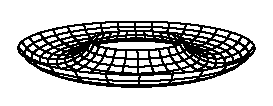
\includegraphics{asy/gutter}
\end{wrapfigure}

%%%%%%%%%%%%%%%%%%%%%%%%%%%%%%%%%%%%%%%%%%%%%%
\subsection*{Round gutter\hard}
\label{half-torus}

A round gutter is the surface shown on the picture.

}

More precisely, consider the torus $T$; a surface generated by revolving a circle in $\RR^3$ around an axis coplanar with the circle.
Let $\gamma\z\subset T$ be one of the circles in $T$ that locally separates positive and negative curvature on $T$;
a plane containing $\gamma$ is tangent to $T$ at all points of $\gamma$.
Then a neighborhood of $\gamma$ in $T$ is called 
\index{gutter}\emph{round gutter}
and the circle $\gamma$ is called its {}\emph{main latitude}.



\begin{pr}
Let $\Omega\subset \RR^3$ be a round gutter with main latitude $\gamma$. 
Assume that $\iota\:\Omega\z\to\RR^3$ 
is a smooth length-preserving embedding that is sufficiently close to the identity.
Show that $\gamma$ and $\iota(\gamma)$ are congruent;
that is, there is an isometric motion of $\RR^3$ sending $\gamma$ to $\iota(\gamma)$
\end{pr}



%%%%%%%%%%%%%%%%%%%%%%%%%%%%%%%%%%%%%%%%%%%%%%
\subsection*{Non-contractible geodesics}
\label{torus}

\begin{pr}
Give an example of a non-flat metric 
on the $2$-torus such that no closed geodesic is contractible.
\end{pr}


%%%%%%%%%%%%%%%%%%%%%%%%%%%%%%%%%%%%%%%%%%%%%%
\subsection*{Two disks}
\label{Two disks}

\begin{pr}
Let $\Sigma_1$ and $\Sigma_2$ be two smoothly embedded open disks in $\mathbb R^3$ 
that have a common closed smooth curve $\gamma$.
Show that there is a pair of points  $p_1\in \Sigma_1$ and $p_2\in \Sigma_2$ with parallel tangent planes.
\end{pr}



\section*{Semisolutions}
%%%%%%%%%%%%%%%%%%%%%%%%%%%%%%%%%%%%%%%%%%%%%%%%%%
\parbf{Involute of  geodesic.}
Let $W$ be the closed unbounded set formed by $\Sigma$ and its exterior points.
Choose $t\in (0,\ell)$;
denote by $\gamma_t$ the concatenation of the line segment $[p_t\gamma(t)]$ and the arc $\gamma|_{[t,\ell]}$.
The key step is to show the following:

\begin{cl}{$({*})$} The curve $\gamma_t$ is a minimizing geodesic in the intrinsic metric induced on $W$.
\end{cl}


Try to prove it before reading further.

\medskip

Let $\Pi_t$ be the tangent plane to $\Sigma$ at $\gamma(t)$.
Consider the curve $\alpha(t)=p_t$.
Note that  
$\alpha(t)\z\in\Pi_t$,
$\alpha'(t)\perp\Pi_t$
and $\alpha'(t)$ points to the side of $\Pi_t$ opposite to $\Sigma$.



It follows that for any $x\in\Sigma$ the function  
\[t\mapsto |x - p_t|
\quad\text{and, therefore,}\quad
t\mapsto |x - p_t|_W\] are non-decreasing;
here $|x - p_t|_W$ stays for the intrinsic distance from $x$ to $p_t$ in $W$.


\begin{wrapfigure}{r}{43 mm}
\vskip-6mm
\centering
\includegraphics{mppics/pic-205}
\end{wrapfigure}

On the other hand, by construction 
\[|q - p_t|_W\le |q - p|_\Sigma;\] 
therefore, from the above 
\[|q - p_t|_W= |q - p|_\Sigma\]
for any $t$.
Hence $(*)$ follows.

Now assume that $q$ is visible from $p_t$ for some $t$;
that is, the line segment $[qp_t]$ intersects $\Sigma$ only at $q$.
From the above, 
$\gamma_t$  coincides with the line segment $[qp_t]$.
On the other hand, $\gamma_t$ contains $\gamma(t)\in\Sigma$, a contradiction.\qeds

This problem is based on an observation used by Anatoliy Milka in the proof of his (beautiful) generalization of the comparison theorem for convex surfaces \cite{milka-geod}.

%%%%%%%%%%%%%%%%%%%%%%%%%%%%%%%%%%%%%%%%%%%%%%%%%%

\begin{wrapfigure}{r}{43 mm}
\vskip-0mm
\centering
\includegraphics{mppics/pic-206}
\end{wrapfigure}

\parbf{Simple geodesic.} 
Look at two combinatorial types of a self-intersection shown in the diagram.
One of them can and the other cannot appear as self-intersections of a geodesic on an unbounded convex surface.
Try to determine which is which before reading further.

\medskip

Let $\gamma$ be a two-sided infinite geodesic in $\Sigma$.
The following is the key statement in the proof.

\begin{cl}{$({*})$}
The geodesic $\gamma$ contains at most one simple loop.
\end{cl}

To prove $({*})$, we use the following observation.

\begin{cl}{$({*}{*})$}
The integral curvature $\omega$ of $\Sigma$ cannot exceed $2\cdot\pi$.
\end{cl}

Indeed, since $\Sigma$ is unbounded and convex,
it surrounds a half-line.
Consider a coordinate system with this half-line as the positive half of its $z$-axis. 
In these coordinates, the surface $\Sigma$ is described as a graph $z=f(x,y)$ of a convex function $f$.
In particular all outer normal vectors to $\Sigma$ have negative $z$-coordinate;
in other words they point to the south hemisphere.
Therefore the area of the spherical image of $\Sigma$ is at most $2\cdot\pi$.
The area of this image is the integral of the Gauss curvature over $\Sigma$. 
Hence $({*}{*})$ follows.

From the Gauss--Bonnet formula, we get the following conclusion.
If $\phi$ is the angle at the base of a simple geodesic loop then the integral curvature surrounded by the loop equals $\pi+\phi$. 
In particular $({*}{*})$ implies that $\phi\le\pi$; in other words, there are no \emph{concave loops}.

Now assume that $({*})$ does not hold, so that a geodesic has two simple loops.
Note that the disks bounded by the loops  have to overlap,
otherwise the curvature of $\Sigma$ would exceed $2\cdot\pi$.
But if they overlap, then it is easy to show that the curve also contains a concave loop, 
which contradicts the above observation.%
\footnote{This observation implies that the right picture on the above diagram cannot be realized by a geodesic.}

If a geodesic $\gamma$ has a self-intersection,
then it contains a simple loop.
From $({*})$, there is only one such loop;
it cuts a disk from $\Sigma$ 
and goes around it either clockwise or counterclockwise.
This way we divide all the self-intersecting geodesics 
into two sets which we will call {}\emph{clockwise} and {}\emph{counterclockwise}.

Note that the geodesic $t\mapsto \gamma(t)$ is clockwise 
if and only if 
$t\z\mapsto \gamma(-t)$
is counterclockwise.
The sets of clockwise and counterclockwise are open and the space of all geodesics is connected. 
It follows that there are geodesics 
which aren't clockwise nor counterclockwise.
Those geodesics have no self-intersections.\qeds

Note that the proof implies that a two-sided infinite geodesic can be found among geodesics containing a given point in $\Sigma$.

The problem is due to Stephan Cohn-Vossen \cite[see Satz 9 in][]{convossen};
generalizations were obtained  by 
Vladimir Streltsov and Alexandr Alexandrov 
\cite{streltsov-alexandrov} 
and 
by Victor Bangert \cite{bangert}.


%%%%%%%%%%%%%%%%%%%%%%%%%%%%%%%%%%%%%%%%%%%%%%%%%%
\parbf{Geodesics for birds.}
Choose a unit-speed geodesic in $W$, say
\[\gamma\:t\mapsto(x(t),y(t),z(t)).\]
We can assume that $\gamma$ is defined on a closed interval $[a,b]$.
The key step is to show the following:

\begin{cl}{$({*})$} 
The function $t\mapsto z$ is concave.
\end{cl}


Parametrize the plane curve $t\mapsto (x(t),y(t))$ by the arc length $s$
and reparametrize $\gamma$ by $s$.

\begin{wrapfigure}{r}{35 mm}
\vskip-4mm
\centering
\includegraphics{mppics/pic-208}
\end{wrapfigure}

Note that the function $s\mapsto z$ is concave.
Indeed, suppose $s\mapsto z$ is not concave around $s_0$.
Then one could shorten $\gamma$ by increasing its $z$ component in a small interval around $s_0$, while keeping its endpoints fixed.
After the deformation, the curve still lies in $W$.
The latter contradicts that $\gamma$ is locally length minimizing.

Finally note that concavity of $s\mapsto z$ is equivalent to the concavity of $t\mapsto z$.
Hence $({*})$ follows.



Since $f$ is smooth, 
the curve $\gamma(t)$ is $C^{1,1}$; 
that is, its first derivative $\gamma'(t)$ is a well defined Lipschitz function.
It follows that its second derivative $\gamma''(t)$ is defined almost everywhere.

Since $z(t)$ is concave, we have $z''(t)\le 0$.
Since $f$ is $\ell$-Lipschitz, $z(t)$ is $\tfrac{\ell}{\sqrt{1+\ell^2}}$-Lipschitz.
It follows that 
\[\int\limits_a^b |z''(t)|\le 2\cdot\tfrac{\ell}{\sqrt{1+\ell^2}}.\]

The curvature vector $\gamma''(t)$ is perpendicular to the surface.
Since the surface has slope at most $\ell$,
we get 
\[|\gamma''(t)|\le |z''(t)|\cdot\sqrt{1+\ell^2}.\]
Hence 
\[\int\limits_a^b |\gamma''(t)|\le 2\cdot\ell.\qedsin\]
\medskip

The statement holds for general $\ell$-Lischitz functions,
not necessarily smooth.
The given bound is optimal, the equality is attained by a two-side infinite geodesic on the graph of  
\[f(x,y)=-\ell\cdot\sqrt{x^2+y^2}.\]

The problem is due to David Berg \cite{berg},
the same bound for convex $\ell$-Lipschitz surfaces was proved earlier by Vladimir Usov \cite{usov}.
The observation $({*})$
is called \index{Liberman’s lemma}\emph{Liberman’s lemma}; 
it was used earlier 
to bound the total curvature
of a geodesic on a convex surface \cite{liberman}.\footnote{It is a part of the thesis of Joseph Liberman, defended a couple of months before his death in WWII.}
This lemma is often useful when working with geodesics on general convex surfaces.

%%%%%%%%%%%%%%%%%%%%%%%%%%%%%%%%%%%%%%%%%%%%%%%%%%
\parbf{Immersed surface.}
Let $\ell$ be a linear function that vanishes on $\Pi$ 
and is positive on $\Sigma$. 
We will apply a Morse type argument for the restriction of $\ell$ to $\Sigma$.

\medskip

Let $z_0$ be a maximum of $\ell$ on $\Sigma$;
set $s_0=\ell(z_0)$.
Given $s<s_0$, denote by $\Sigma_s$ the connected component of $z_0$ in $\Sigma\cap\ell^{-1}([s,s_0])$.
Note that for all $s$ sufficiently close to $s_0$
we have
\begin{itemize}
\item $\Sigma_s$ is an embedded disk;
\item $\partial\Sigma_s$ is a convex plane curve.
\end{itemize}

Consider the set $A\subset [0,s_0)$ such that for any $a\in A$ these two conditions hold for any $s\in [a,s_0)$.
Observe that $A$ is open and closed in $[0,s_0)$.
Whence $A=[0,s_0)$; in particular, these conditions hold for $s=0$.

Since $\Sigma$ is connected, $\Sigma_0=\Sigma$.
Hence the result follows.\qeds

This problem is discussed in the lectures of Mikhael Gromov \cite[see \S$\tfrac12$~in][]{gromov-SGMC}.

%%%%%%%%%%%%%%%%%%%%%%%%%%%%%%%%%%%%%%%%%%%%%%%%%%
\parbf{Periodic asymptote.}
Arguing by contradiction, assume that there is a geodesic $\gamma$ on the surface $\Sigma$ with a periodic asymptote $\delta$. 

Passing to a finite cover of $\Sigma$, we can ensure that the asymptote has no self-intersections.
In this case, 
the restriction $\gamma|_{[a,\infty)}$  
has no self-intersections 
if $a$ is sufficiently large.

Cut $\Sigma$ along $\gamma([a,\infty))$ and then cut from the obtained surface an infinite triangle $\triangle$. 
The triangle $\triangle$ has two sides formed by both sides of cuts along $\gamma$;
let us denote these sides of $\triangle$ by $\gamma_-$ and $\gamma_+$.
Note that 
\[\area\triangle<\area \Sigma<\infty\leqno(*)\]
and both sides $\gamma_\pm$ 
are infinite minimizing geodesics in $\triangle$.

Consider the Busemann function $f$ for $\gamma_+$ [defined on page~\pageref{page:Busemann function}];
denote by $\ell(t)$ the length of the level curve $f^{-1}(t)$.
Let $-\kappa(t)$  be the total curvature of the sup-level set $f^{-1}([t,\infty))$.  
From the Gauss--Bonnet formula,
\[\ell'(t)=\kappa(t).\leqno({*}{*})\]

The level curve $f^{-1}(t)$ can be parametrized by a unit-speed curve, say $\theta_t\:[0,\ell(t)]\to \triangle$.
By the coarea formula we have
\[\kappa'(t)
=
-\int\limits_0^{\ell(t)} K_{\theta_t(\tau)}\cdot d\tau,
\]
where $K_x$ denotes the Gauss curvature of $\Sigma$ at the point $x$.
Since $K_{\theta_t(0)}\z=K_{\theta_t(\ell_t)}=0$ and the surface is smooth,
there is a constant $C$ such that $|K_{\theta_t(\tau)}|\le C\cdot \ell(t)^2$ for all $t$, $\tau$.
Therefore
\[\kappa'(t)\le C\cdot \ell(t)^3 \leqno(\asterism)\]

Together, $({*}{*})$ and $(\asterism)$ imply that there is $\eps>0$ such that
\[\ell(t)\ge \frac\eps{t-a}\]
for sufficiently large $t$.
By the coarea formula we get 
\[\area\triangle=\int\limits_a^\infty\ell(t)=\infty;\]
the latter contradicts $(*)$.\qeds

I learned the problem from 
Dmitri Burago 
and Sergei Ivanov, 
it originated from a discussion with
Keith Burns, 
Michael Brin 
and Yakov Pesin.

Here is a motivation.
Let $\Sigma$ be a closed surface with non-positive curvature that is not flat.
The space $\Gamma$ of all unit-speed geodesics $\gamma\:\RR\z\to\Sigma$ can be identified with the unit tangent bundle $\UU\Sigma$. 
In particular $\Gamma$ comes with a natural choice of measure.
Denote by $\Gamma_0\subset \Gamma$ the set of geodesics that run in the set of zero curvature all the time.
It is expected that $\Gamma_0$ has vanishing measure.
In all known examples $\Gamma_0$ contains only periodic geodesics in only finitely many homotopy classes \cite[see also][]{hertz}.

%%%%%%%%%%%%%%%%%%%%%%%%%%%%%%%%%%%%%%%%%%%%%%%%%%
\parbf{Saddle surface.}
Denote by $\Sigma^\circ$ the interior of $\Sigma$.
Choose a plane $\Pi$. 
Note that the intersection $\Pi\cap \Sigma^\circ$ 
locally looks either like a curve or like two curves intersecting transversally;
in the latter case $\Pi$ is tangent to $\Sigma^\circ$ at the intersection point.

Further note that $\Pi\cap \Sigma^\circ$ has no cycle.
Otherwise $\Sigma$ would fail to be saddle at the point of the disk surrounded by that cycle maximizing the distance to $\Pi$.

If $\Sigma$ is not a graph then there is a point $p\in\Sigma$ with a vertical tangent plane;
denote this plane by $\Pi$.
The intersection $\Pi\cap\Sigma$ has cross-point at~$p$.

Since the boundary of $\Sigma$ projects injectively to a closed convex curve in $(x,y)$-plane,
the intersection of $\Pi\cap\partial \Sigma$ has at most 2 points --- these are the only endpoints of $\Pi\cap\Sigma$.

It follows that the connected component of $p$ in $\Pi\cap\Sigma$ is a tree 
with a vertex of degree 4 at $p$ and at most two end-points, a contradiction.\qeds

The described idea can be used to prove the result of Richard Schoen and Shing-Tung  Yau \cite{schoen-yau-2D} which gives a sufficient condition for a harmonic map between surfaces to be a diffeomorphism.
Unlike the original proof, it requires no calculations.

The proof above is based on the observation 
that for any saddle surface $\Sigma$ and plane $\Pi$,
each connected component of $\Sigma\backslash \Pi$ is either unbounded or intersects the boundary curve.
This observation plays a central role in the proof of Sergei Bernstein \cite{bernshtein}
of the following problem:

\begin{pr}
Show that a smooth bounded function $f\:\RR^2\to\RR$ cannot have a strictly saddle graph.
\end{pr}

One could go further and define a \emph{generalized saddle surface} as an arbitrary (non necessarily smooth) surface satisfying the observation above.
The geometry of these surfaces is far from being understood,
Samuil Shefel has a number of beautiful results about them, 
\cite[see][and the references therein]{shefel, AKP-invitation}.
The statement of the problem holds for these generalized saddle surfaces, but
the proof is tricky \cite{petrunin-stadler}.


%%%%%%%%%%%%%%%%%%%%%%%%%%%%%%%%%%%%%%%%%%%%%%%%%%
\parbf{Asymptotic line.}
Denote by $\Pi_t$ the tangent plane to $\Sigma$ at $\gamma(t)$ and by $\ell_t$ the tangent line of $\gamma$ at time $t$.

Since $\gamma$ is asymptotic, the plane $\Pi_t$ rotates around $\ell_t$ as $t$ changes.
Since $\Sigma$ is saddle, the speed of rotation cannot vanish.%
\footnote{By the Beltrami--Enneper theorem, if $\gamma$ has unit speed, then the speed of rotation is $\pm\sqrt{-K}$, where $K$ is the Gauss curvature which cannot vanish on a saddle surface.}

Note that $\Pi_t$ is a graph of a linear function, say $h_t$, defined on the $(x, y)$-plane.
Denote by $\bar\ell_t$ the projection of $\ell_t$ to the $(x, y)$-plane.
The described rotation of $\Pi_t$ can be expressed algebraically:
the derivative $\tfrac{d}{dt}h_t(w)$ vanishes at the point $w$ if and only if $w\in \bar\ell_t$ 
and the derivative changes sign if $w$ changes the side of $\bar\ell_t$.

Denote by $\bar\gamma$ the projection of $\gamma$ to the $(x, y)$-plane.
If $\bar\gamma$ is star shaped with respect to a point $w$, then $w$ cannot cross $\bar\gamma_t$.
Therefore the function $t\mapsto h_t(w)$ is monotone on $\SSS^1$.
Observing that this function cannot be constant, we arrive at a contradiction.\qeds

The problem is discussed by Dmitri Panov \cite{panov-curves}.

%%%%%%%%%%%%%%%%%%%%%%%%%%%%%%%%%%%%%%%%%%%%%%%%%%
\parbf{Minimal surface.}
Without loss of generality we may assume that the sphere is centered at the origin of $\RR^3$.

Let $h$ be the restriction of the function $x\mapsto \tfrac12\cdot|x|^2$ to the surface $\Sigma$.
Direct calculations show that $\Delta_\Sigma h =  2$;
here $\Delta_\Sigma$ denoted Laplacian on $\Sigma$.
Applying the divergence theorem for the gradient $\nabla_\Sigma h$
in $\Sigma_r\z=\Sigma\cap B(0,r)$, we get
\[2\cdot \area\Sigma_r\le r\cdot\length [\partial\Sigma_r].\]

Set $a(r)=\area\Sigma_r$.
By the coarea formula, $a'(r)\ge\length [\partial\Sigma_r]$ for almost all $r$.
Therefore the function
\[f\:r\mapsto \frac{\area\Sigma_r}{r^2}
\]
is non-decreasing in the interval $(0,1)$.

Since $f(r)\to \pi$ as $r\to0$, the result follows.\qeds

We described a partial case of the so-called \index{monotonicity formula}\emph{monotonicity formula} for minimal surfaces.

The same argument shows that if $0$ is a double point
of $\Sigma$ then $\area\Sigma\z\ge 2\cdot \pi$.
This observation was used to prove 
that the minimal disk bounded by a simple closed curve with total curvature $\le 4\cdot\pi$ 
is necessarily embedded.
It was proved by 
Tobias Ekholm, 
Brian White 
and Daniel Wienholtz
\cite{EWW};
an amusing variation of this proof
was obtained by 
Stephan Stadler \cite{stadler-FM}.
This result also implies that any embedded circle of total curvature at most $4\cdot\pi$ is unknot.
The latter was proved independently by Istv{\'a}n F{\'a}ry \cite{fary-knot} and  John Milnor \cite{milnor}.

Note that if we assume in addition that the surface is a disk,
then the statement holds for any saddle surface. 
Indeed, denote by $S_r$ the sphere of radius $r$ concentrical with the unit sphere. 
Then according to the problem ``A curve on a sphere'' [page \pageref{A curve in a sphere}], 
\[\length[\partial\Sigma_r]\ge 2\cdot\pi\cdot r.\]
Then by the coarea formula we get $\area\Sigma\ge \pi$.

On the other hand, there are saddle surfaces homeomorphic to the cylinder
having an arbitrarily small area in the ball. 

If $\Sigma$ does not pass thru the center 
and we only know the distance, say $r$, 
from the center to $\Sigma$,
then the optimal bound is $\pi\cdot(1-r^2)$.
This question was open for about 40 years and proved by Simon Brendle and Pei-Ken Hung \cite{brende-hung};
their proof is based on a similar idea and is quite elementary.
Earlier Herbert Alexander, 
David Hoffman
and Robert Osserman 
proved it for two cases: (1) for disks and (2) for arbitrary area minimizing surfaces, any dimension and codimension
 \cite{alexander-osserman,alexander-hoffman-osserman}.






%%%%%%%%%%%%%%%%%%%%%%%%%%%%%%%%%%%%%%%%%%%%%%%%%%
\parbf{Round gutter.}
Without loss of generality, we can assume that the length of $\gamma$ is $2{\cdot}\pi$ and its intrinsic curvature is $1$ at all points.

Let $K$ be the convex hull of $\hat\Omega=\iota(\Omega)$.
Part of $\hat\Omega$ touches the boundary of $K$ and the rest lies in the interior of $K$. 
Denote by $\hat\gamma$ the curve in $\hat\Omega$ dividing these two parts.

First note that the Gauss curvature of $\hat\Omega$ should vanish at the points of $\hat\gamma$;
in other words, $\hat\gamma=\iota(\gamma)$.
Indeed, since $\hat\gamma$ lies on the convex part, 
the Gauss curvature at the points of $\hat\gamma$ should be non-negative. 
On the other hand, $\hat\gamma$ bounds a flat disk in $\partial K$;
therefore its integral intrinsic curvature should be $2{\cdot}\pi$.
If the Gauss curvature is positive at some point of $\hat\gamma$, 
then by the Gauss--Bonnet formula, the total intrinsic curvature of $\hat\gamma$ should be smaller than $2{\cdot}\pi$, a contradiction.

On the other hand, $\hat\gamma$ is an asymptotic line.
Indeed, if the direction of $\hat\gamma$ is not asymptotic at some $t_0$,
then $\hat\gamma(t_0 \pm\eps)$ lies the interior of $K$ for some small $\eps>0$, a contradiction.

Therefore, as the space curve,
$\hat\gamma$ has to be a closed curve with constant curvature $1$.
Any such curve is congruent to a unit circle.\qeds

It is not known whether $\hat\Omega$ is congruent to $\Omega$ or not.

The solution presented above is based on my answer 
to the question of Joseph O'Rourke \cite{rourke}.
Here are some related statements.
\begin{itemize}
\item A gutter is second order rigid;
this was proved by Eduard Rembs
[see \ncite{rembs} and also page 135 in \ncite{efimov}].
\item Any second order rigid surface does not admit analytic deformation 
[proved by Nikolay Efimov; page 121 in \ncite{efimov}]
and for the surfaces of revolution, the assumption of analyticity can be removed 
\cite[proved by Idzhad Sabitov, see][]{sabitov}.
\end{itemize}









%%%%%%%%%%%%%%%%%%%%%%%%%%%%%%%%%%%%%%%%%%%%%%%%%%
\parbf{Non-contractible geodesics.}
A torus of revolution is an example.

Indeed, it has a family of {}\emph{meridians} --- a family of circles that form closed geodesics.
Note that a geodesic on the torus is either a meridian
or it intersects meridians transversally.
In the latter case all the meridians are crossed by the geodesic in the same direction.

Note that a contractible curve has to cross each meridian an equal number of times in both directions.
Therefore no geodesic of the torus is contractible.\qeds 


I learned this problem 
from the book of Mikhael Gromov \cite{gromov-MetStr},
where it is attributed to Y. Colin de Verdi\`ere.
The same argument can be used to show that a torus with a geodesic foliation has no contractible closed geodesics.
I do not know other examples of that type \cite{petrunin-torus}; namely the following question is open:

\begin{pr}
Are there examples of Riemannian metrics on the 2-torus without closed null-homotopic geodesics and without a geodesic foliation?
\end{pr}


%%%%%%%%%%%%%%%%%%%%%%%%%%%%%%%%%%%%%%%%%%%%%%%%%%
%%%%%%%%%%%%%%%%%%%%%%%%%%%%%%%%%%%%%%%%%%%%%%%%%%
\parbf{Two disks.}
Choose a continuous map $h\:\Sigma_1\to \Sigma_2$
that is the identity on $\gamma$.
Let us prove that for some $p_1\in \Sigma_1$ and $p_2=h(p_1)\in \Sigma_2$,
the tangent planes $\T_{p_1} \Sigma_1$ and  $\T_{p_2} \Sigma_2$ are parallel;
this fact is stronger than the one required.

\medskip

Arguing by contradiction,
assume that such a point does not exist.
Then for each $p\in\Sigma_1$
there is a unique line $\ell_p\ni p$ 
 parallel to both $\T_{p} \Sigma_1$ and $\T_{h(p)} \Sigma_2$.

Note that the lines $\ell_p$ form a tangent line distribution over $\Sigma_1$
and $\ell_p$ is tangent to $\gamma$ at all $p\in\gamma$.

Let $\Delta$ be the disk in $\Sigma_1$ bounded by $\gamma$.
Consider the doubling of $\Delta$ along  $\gamma$;
it is diffeomorphic to $\mathbb S^2$.
The line distribution $\ell$ lifts to a line distribution on the doubling.
The latter contradicts the hairy ball theorem.\qeds


This proof was suggested nearly simultaneously 
by Steven Sivek 
and Damiano Testa \cite{two-disks}.

Note that the same proof works when $\Sigma_i$ are oriented open surfaces and $\gamma$ cuts a compact domain in each $\Sigma_i$.

There are examples of three disks $\Sigma_1$, $\Sigma_2$ and $\Sigma_3$
with a common closed curve $\gamma$ such that there is
no triple of points $p_i\in\Sigma_i$ with parallel tangent planes.
Such examples can be found among ruled surfaces \cite{three-disks}.
